\documentclass[12pt]{article}
\usepackage{bbm}
\usepackage{fancyhdr}
\usepackage{titling}
\usepackage{enumitem}
\usepackage{amsmath}
\usepackage{dsfont}
\usepackage{amsfonts}
\usepackage{amssymb}
\usepackage{amsthm}
\usepackage{geometry}
\usepackage{tikz}
\usepackage{algorithm}
\usepackage{algpseudocode}
\geometry{verbose,tmargin=1in,bmargin=1in,lmargin=1in,rmargin=1in}
\renewcommand{\vec}[1]{\mathbf{#1}}
\newcommand{\dec}{\text{dec}}
\newcommand{\divi}{\mathbin{\textnormal{div}}}
\title{Homework 1}
\author{Satvik Prasad}
\date{}
\newtheorem{lemma}{Lemma}[section]
\fancypagestyle{plain}{%
  \fancyhf{}
  \fancyhead[L]{\theauthor}
  \fancyhead[R]{\thedate}
}
\pagestyle{plain}
\makeatletter
\def\@maketitle{%
  \newpage
  \null
  \vskip 1em%
  \begin{center}%
    \let \footnote \thanks
    {\LARGE \@title \par}%
    \vskip 1em%
  \end{center}%
  \par
\vskip 1em}
\makeatother
\usepackage{cmbright}

\newcommand{\mat}[1]{\mathbf{#1}}

% ---------- Probability theory ----------
% Core operators (optional argument-free; use as \E{X}, \Var{X}, \Cov{X}{Y})
\DeclareMathOperator{\EOp}{\mathbb{E}}
\DeclareMathOperator{\VarOp}{Var}
\DeclareMathOperator{\CovOp}{Cov}
\DeclareMathOperator{\CorrOp}{Corr}

\renewcommand{\P}[1]{\mathbb{P}\left(#1\right)}        % \P{A}
\newcommand{\E}[1]{\EOp\left[#1\right]}                % \E{X}
\newcommand{\Var}[1]{\VarOp\left(#1\right)}            % \Var{X}
\newcommand{\Cov}[2]{\CovOp\left(#1,\,#2\right)}       % \Cov{X}{Y}
\newcommand{\Corr}[2]{\CorrOp\left(#1,\,#2\right)}     % \Corr{X}{Y}
\newcommand{\SD}[1]{\operatorname{SD}\left(#1\right)}  % \SD{X}

% Subscripted versions, e.g. \Esub{\theta}{X}, \Psub{\theta}{A}
\newcommand{\Esub}[2]{\EOp_{#1}\left[#2\right]}
\newcommand{\Psub}[2]{\mathbb{P}_{#1}\left(#2\right)}

% Conditioning, indicators, independence
\newcommand{\given}{\,\middle|\,}                      % \E{X \given Y}
\newcommand{\ind}[1]{\mathbbm{1}\left\{#1\right\}}     % \ind{X > 0}
\newcommand{\indep}{\perp\!\!\!\perp}                  % X \indep Y
\newcommand{\iid}{\overset{\text{iid}}{\sim}}          % X_i \iid \Normal(0,1)

% Convergence
\newcommand{\convp}{\xrightarrow{\;p\;}}               % in probability
\newcommand{\convd}{\xrightarrow{\;d\;}}               % in distribution
\newcommand{\convas}{\xrightarrow{\text{a.s.}}}        % almost surely
\newcommand{\convLp}[1]{\xrightarrow{L^{#1}}}          % in L^p

% Probability spaces
\newcommand{\F}{\mathcal{F}}                           % sigma-algebra
\newcommand{\B}{\mathcal{B}}                           % Borel sigma-algebra
\newcommand{\pspace}{(\Omega, \F, \mathbb{P})}

% Common distributions
\newcommand{\Normal}{\mathcal{N}}
\newcommand{\Bern}{\operatorname{Bernoulli}}
\newcommand{\Bin}{\operatorname{Binomial}}
\newcommand{\Pois}{\operatorname{Poisson}}
\newcommand{\Unif}{\operatorname{Uniform}}
\newcommand{\Exp}{\operatorname{Exp}}
\newcommand{\Geom}{\operatorname{Geometric}}
\newcommand{\Gam}{\operatorname{Gamma}}
\newcommand{\Beta}{\operatorname{Beta}}

% Number sets
\newcommand{\R}{\mathbb{R}}
\newcommand{\N}{\mathbb{N}}
\newcommand{\Z}{\mathbb{Z}}


\begin{document}
\subsection{Writing Proofs}
\begin{enumerate}
    \item Let $U^{\infty}$ denote $$\bigcap_{\alpha \in S} U_{\alpha}.$$ We now need to prove it is closed under scalar addition, scalar multiplication, and contains the additive identity.

    \begin{itemize}
        \item Consider $f \in U^{\infty}$ and $g \in U^{\infty}.$ By definition, this means $f, g \in U_{\alpha}$ for all $\alpha \in S.$ Since $U_{\alpha}$ is a subspace, $f + g$ is also in $U_{\alpha},$ meaning $f + g \in U_{\alpha}$ for all $\alpha \in S.$ Thus, by the definition of $U^{\infty},$ $f + g \in U^{\infty},$ meaning $U^{\infty}$ is closed under addition.
        \item Consider an arbitrary $f \in U^{\infty}.$ Then, $f \in U_{\alpha}$ for all $\alpha \in S.$ Since $U_\alpha$ is closed under scalar multiplication, $$\lambda f \in U_\alpha$$ for all $\alpha \in S,$ meaning by definition $\lambda f \in U^{\infty},$ and hence $U^{\infty}$ is closed under scalar multiplication.

        \item $0,$ the additive identity of $V,$ must be contained in $U_\alpha$ for all $\alpha \in S$ since $U_\alpha$ is a subspace, meaning by definition $0 \in U^{\infty}.$

        \item Finally, since $U_{\alpha}$ is a subset of $V,$ by the definition of the intersection, $U^{\infty}$ is a subset of $V.$
    \end{itemize}

    Thus, because $U^{\infty}$ satisfies the above criteria, it is a subspace of $V.$

    \item Counterexample: $V = \mathbb R^{2},$ $U = \{(x, 0) : x \in \mathbb R \},$ $V_1 = \{(x, y) : y = -x\},$ and $V_2 = \{(x, y) : y=x\}.$ This is because $U$ and $V_1$ have a direct sum of $V$, $U$ and $V_2$ have a direct sum $V,$ but $V_1 \neq V_2.$

    \item Since $v_1, v_2, v_3, v_4$ span $V,$ we know that for all $v \in V,$ there exists $\lambda_i \in \mathbb F$ such that \begin{align*}
        \lambda_1 v_1 + \lambda_2 v_2 + \lambda_3 v_3 + \lambda_4 v_4 = v. 
    \end{align*}
    Then, consider $\mu_1, \ldots, \mu_4 \in \mathbb F$ such that \begin{align*}
            v_0 = \mu_1 (v_1 - v_2) + \mu_2(v_2 -v _3) + \mu_3(v_3 - v_4) + \mu_4 v_4.
    \end{align*}
    Distributing, we get \begin{align*}
        v_0 = \mu_1 v_1 + (\mu_2 - \mu_1)v_2 + (\mu_3 - \mu_2) v_3 + (\mu_4 - \mu_3) v_4
    \end{align*}

    Consider an arbitrary $v \in V$ defined by a linear combination of $v_1, v_2, \ldots, v_4$ with coefficients $\lambda_1, \lambda_2, \ldots, \lambda_4.$ Then, for $v = v_0,$ there exist coefficients $\mu$ \begin{align*}
        \mu_1 = \lambda_1, \qquad   \mu_2 = \lambda_2 + \lambda_1, \qquad \mu_3 = \lambda_3 + \lambda_2 + \lambda_1, \qquad \mu_4 = \lambda_1 + \lambda_2 + \lambda_3 + \lambda_4
    \end{align*}
    are coefficients such that \begin{align*}
        \mu_1(v_1 - v_2)  + \mu_2(v_2 - v_3) + \mu_3 (v_3 - v_4) + \mu_4 v_4 = v.
    \end{align*}
    Therefore, by definition $\text{span}\{v_1 - v_2, v_2 -v_3, v_3 - v_4, v_4\} = V$  as required.

    \item No, since $1 - i = -i(1 + i),$ meaning $\{1 - i, 1 + i\}$ are not linearly independent over $\mathbb C.$

    To prove that they're linearly independent over $\mathbb R,$ assume they are not linearly independent, i.e there is a $\lambda \in \mathbb R$ such that $(1 - i) = \lambda (1 + i).$ Then, \begin{align*}
    \lambda = \dfrac{1 -i}{1 + i} = (1 - i)^2 / 2 = -i \not \in \mathbb R,
    \end{align*}
    which is a contradiction. Thus, $\{1 + i, 1 - i\}$ are linearly independent on $\mathbb R.$

    \item False, consider the list $\{v_1, v_2\} = \{\langle 1, 0\rangle, \langle 0, 1\rangle\}$ and $\{w_1, w_2\} = \{\langle 0, 1\rangle, \langle 1, 0 \rangle\}$ on $\mathbb R^2.$ The lists themselves are linearly independent, but $\{v_1 + w_1, v_2 + w_2\} = \{\langle 1, 1 \rangle, \langle 1, 1 \rangle\}$ is not linearly independent, since \begin{align*}
        \langle 1, 1\rangle - \langle 1, 1\rangle = \vec 0.
    \end{align*}
\end{enumerate}
\subsection{Evaluating Proofs}
When we have $\lambda(a_1 v_1 + a_2 v_2 + \ldots + a_m v_m) = 0,$ either $\lambda = 0$ or $a_1 v_1 + \ldots + a_m v_m,$ so we can't immediately conclude that $a_1 v_1 + \ldots + a_m v_m = 0.$

\subsection{Using Computers}
\begin{center}
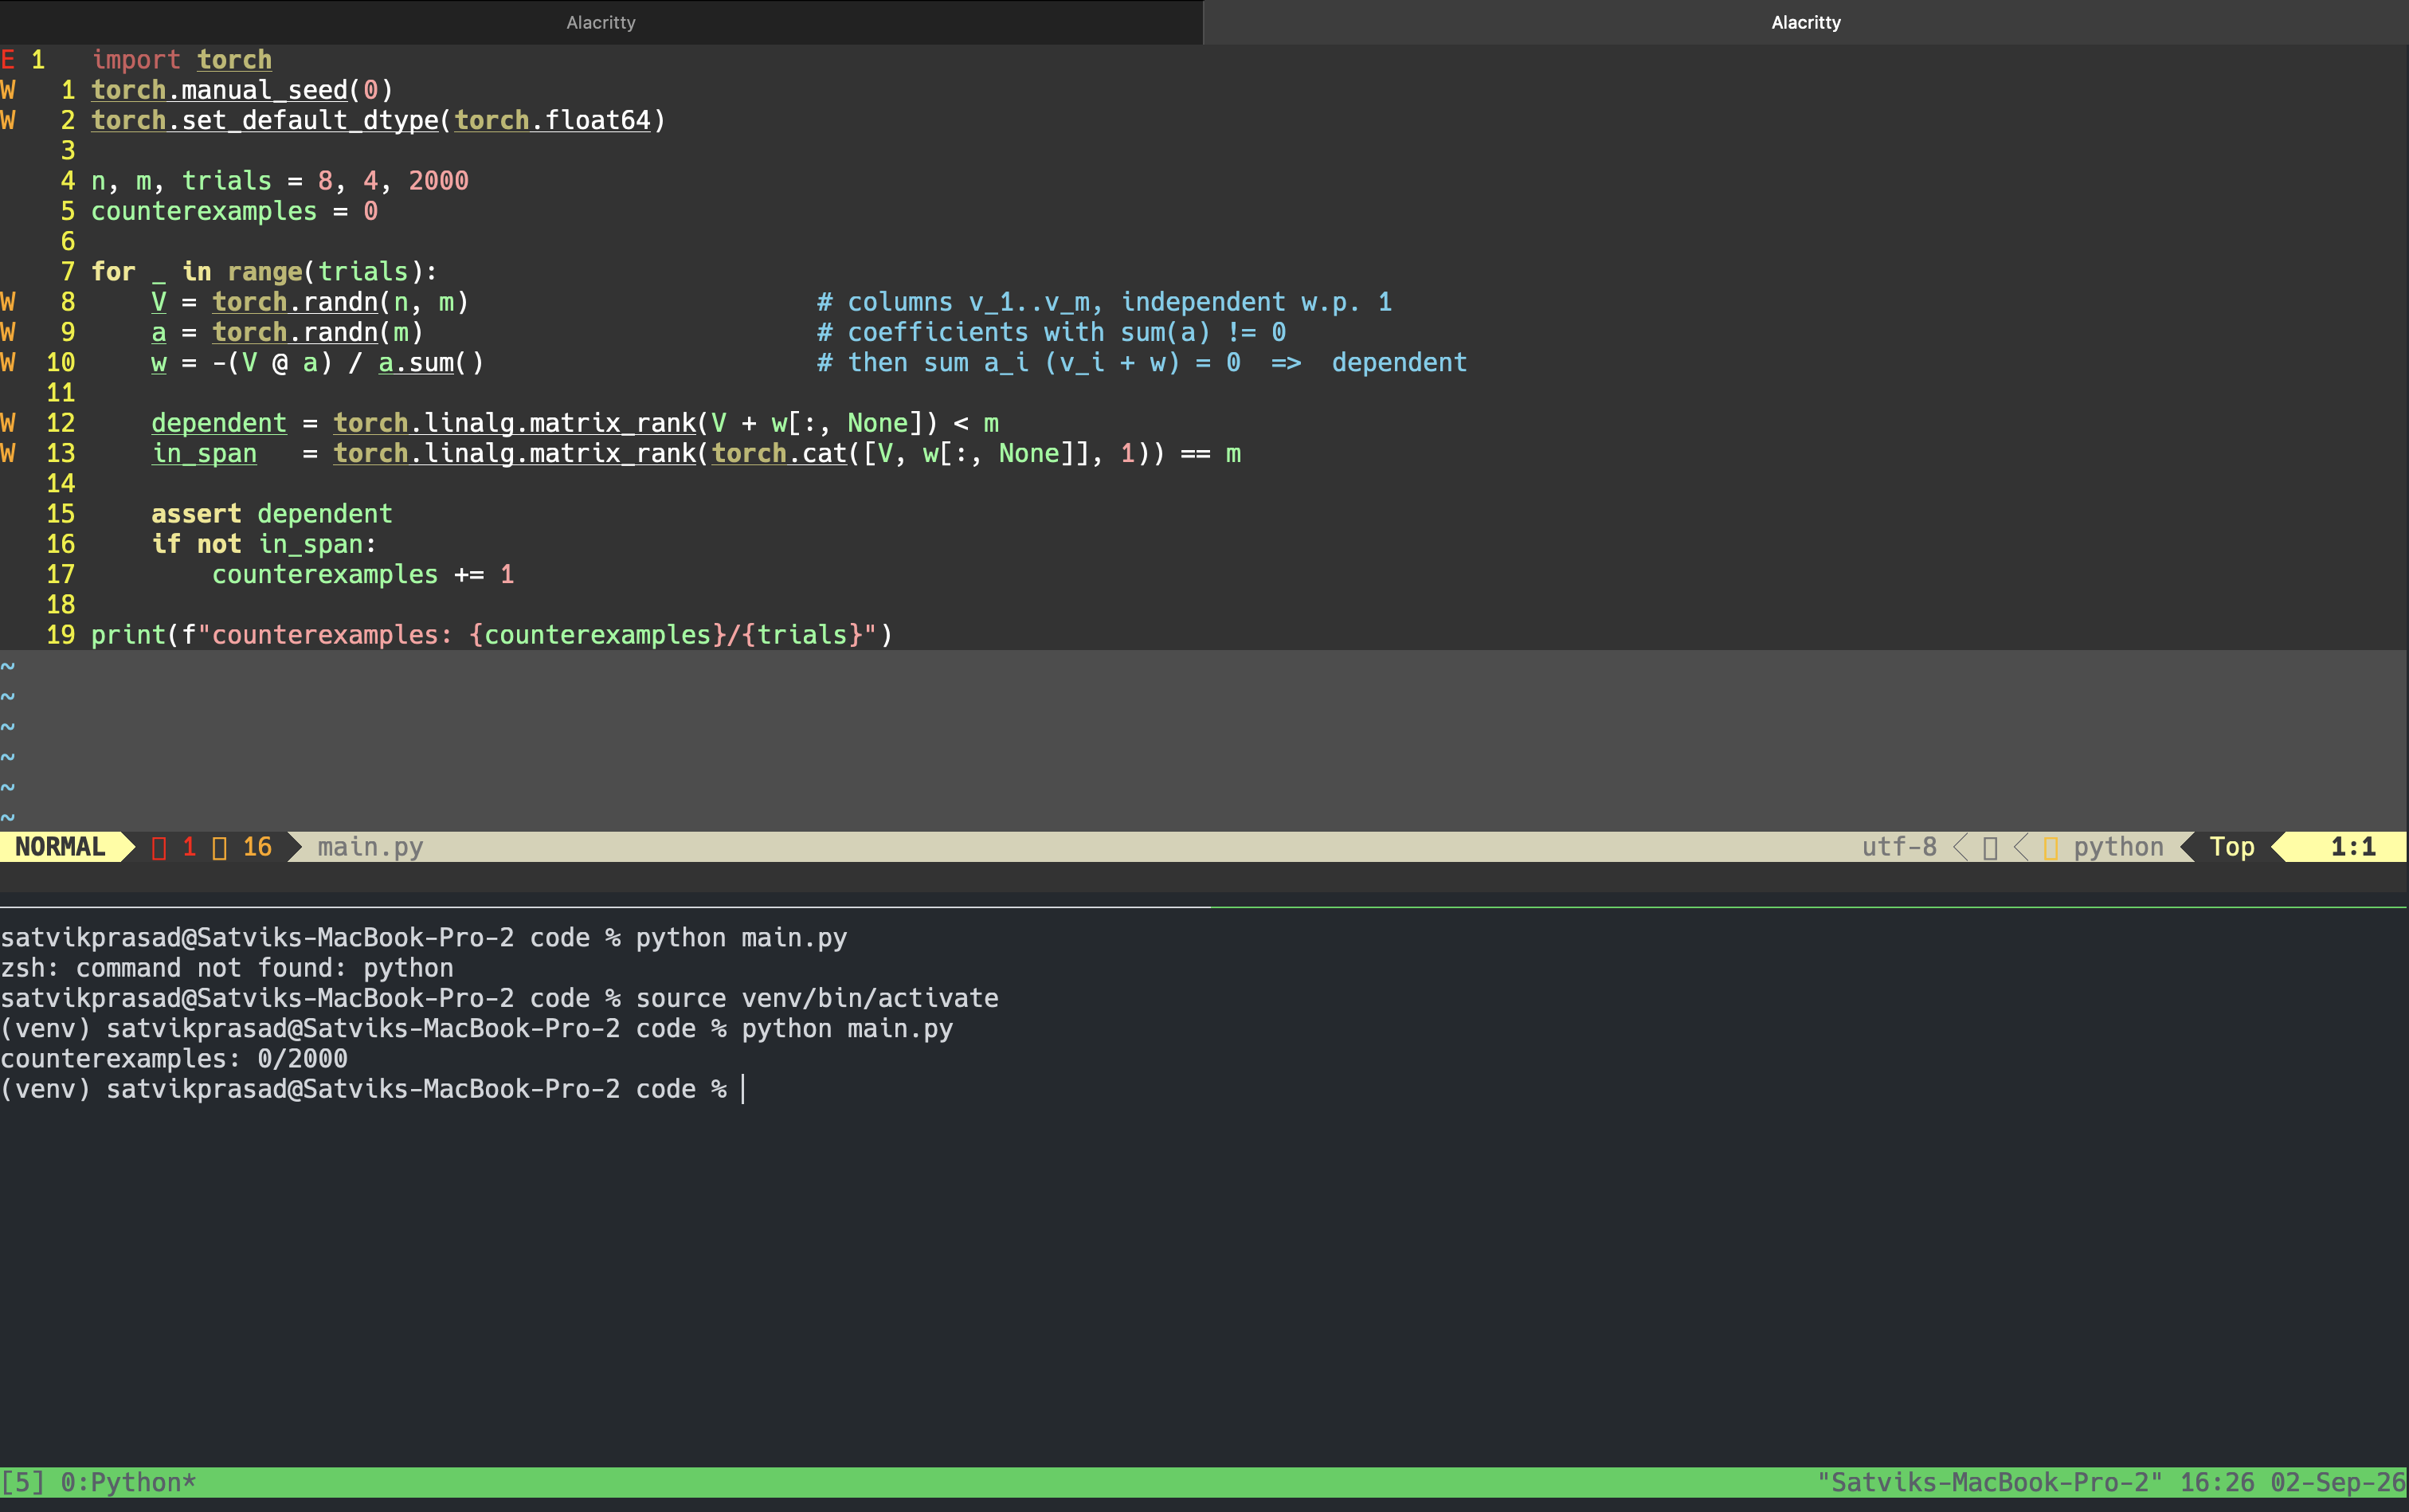
\includegraphics[width=0.9\linewidth]{math3406/Screenshot 2026-09-02 at 4.26.06 pm.png}
\end{center}

The claim is true. Assume we have linearly independent $v_1, v_2, \ldots, v_n \in V,$ and $w \in V$ such that $v_1 + w, \ldots, v_n + w$ are not linearly independent. Then, there are some $\lambda_i$ not all $0$ such that \begin{align*}
\lambda_1 (v_1 + w) + \lambda_2(v_2 + w) + \ldots + \lambda_n (v_n + w) &= 0 \\ \Rightarrow \lambda_1 v_1 + \lambda_2 v_2 + \ldots \lambda_n v_n + (\lambda_1 + \ldots + \lambda _n) w &= 0,
\end{align*}
meaning \begin{align*}
w = -\dfrac{\lambda_1 v_1 + \lambda_2 v_2 + \ldots + \lambda_n v_n}{\underbrace{\lambda_1 + \lambda_2 + \ldots + \lambda_n}_{\neq 0}} .   
\end{align*}
Letting $\mu_i = -\dfrac{\lambda_i}{\lambda_1 + \ldots +\lambda_n},$ where there is at least one $\mu_i$ that is non-zero, we see that \begin{align*}
w = \mu_1 v_1 + \ldots + \mu_n v_n,
\end{align*}
meaning $w $ is in the span of $v_1, \ldots, v_n.$
\end{document}